\section*{Availability-led acquisition and observational velocity inversion}

This update separates live retrieval from the frozen scientific checkpoint. Availability receipts identify 26 candidate stations with public data and 8 with no data returned for the requested bands. The station list contains 51 released identifiers; its membership is not silently equated with the paper's 48 instruments. The observational scope remains incomplete.

At 2026-10-15T17:31:54.283801+00:00, stored coverage is 14,544.383 union channel-hours. Newly acquired observations contribute 1,059.305 channel-hours and 840.7 MB. These totals count actual miniSEED trace intervals, not advertised availability or queued requests. The frozen processing checkpoint uses 1,327 eligible files and 14,080.521 processed channel-hours. Later downloads are recorded separately until processed.

\subsection*{Scope, storage and availability}

The requested period is 21 January 2022 through 20 March 2025, inclusive. HH/EH channels are selected from permitted station metadata. Detailed FDSN availability, rather than earliest/latest extents, is intersected with that period and compared with the union of stored traces. The legacy ledger is classified separately; its entries are requests, not files. Whole-file checksums and trace identifiers detect duplicates; overlapping intervals count once. Existing event-selected snippets remain excluded.

The fixed reserve is 40 GiB, exceeding both the existing 20 GiB guard and 20 percent of initially free space. Retrieval keeps an additional 8 GiB above that reserve for processing outputs. The seven representative files used 74.0 MB and added 91.643 channel-hours. Their measured byte rate implies approximately 0.98 TB for remaining advertised intervals, compared with 103.0 GB initially usable above the reserve. This extrapolation is uncertain across instruments and epochs; it is updated during retrieval.

Requests use two workers, six-hour station/band cores and 30-second context. The ledger retains successful, empty, failed and pending states separately. The byte reserve is checked while streaming. Calendar-month rotation spreads coverage if storage fills. A common 1 December 2024, 00:00--06:00 UTC window is prioritized because the four public 2I stations began recording in November and were absent from training. This calendar choice does not use an earthquake catalog. A controlled collector restart and incomplete, unprocessed transfers are documented in collector\_handoff.json.

EIDA returned no requested-band availability for V0106, CDOV, CROS, CASE, V0102, V0105, V0104, CMDP. This is not proof that no recordings exist elsewhere. RAN and inaccessible local recordings remain separate deferred inputs; no credentials or restricted access were requested. Exact Calo--Tramelli values are not required for these provisional experiments and were not sought.

\par{\footnotesize\path{data/availability_extension/station_crosswalk.csv}}

\par{\footnotesize\path{data/availability_extension/response_epochs.csv}}

\par{\footnotesize\path{data/availability_extension/availability_receipts.json}}

\par{\footnotesize\path{data/availability_extension/legacy_ledger_classification.csv.gz}}

\par{\footnotesize\path{data/availability_extension/station_channel_month.csv}}

\par{\footnotesize\path{data/availability_extension/remaining_available_intervals.csv}}

The frozen cohort has 1,327 file paths, including 10 rows in byte-identical pairs. Five new downloads repeated earlier complete files while testing advertised internal gaps; they added no union coverage. Trace overlap totals 403.573 channel-hours and is counted once. The ledger subsequently excluded 88 already-successful whole-window requests, whose 0.140511 advertised gap channel-hours remain unverified. They are neither covered observations nor demonstrated absences. Fresh unattempted windows continue. Duplicate checks do not certify equality of every partially overlapping sample.

\par{\footnotesize\path{data/availability_extension/catalog_december/overlap_check.json}}

\par{\footnotesize\path{data/availability_extension/prior_success_reconciliation.json}}

\subsection*{What the expanded processing changed}

The frozen expanded checkpoint contains 256,720 picks (42,089 P; 214,631 S), 3,296 provisional associations and 31,096 assigned phases. Relative to the previous checkpoint it adds 10,052 picks. The earliest nine-file extension added 1,340 picks without changing assigned arrivals; its identity check is retained in catalog/association\_change\_check.json. Later checkpoints are distinct, and the calibration counts below are read from the selected current fit.

\par{\footnotesize\path{data/availability_extension/catalog_december/processing_checkpoint.json}}

\par{\footnotesize\path{data/availability_extension/catalog_december/association_change_check.json}}

Although assigned arrival values were unchanged, equal-time arrivals changed row order in CNV input when unrelated picks were appended. The large-cohort inversion then followed a different numerical path. Canonical event/station/phase/time sorting removes that serialization dependence; both calibration inputs now have the same checksum. The sensitivity suite was rerun after this correction. Reproducible input order does not cure the failed scientific validation.

\par{\footnotesize\path{data/availability_extension/phase_order_validation.json}}

\subsection*{Effect of the common December window}

The 1 December 2024 window has 21 stations, 63 channels and 377.977 processed channel-hours. The other five stations with availability elsewhere have no advertised data in this window. Relative to the prior catalog, 3,271 event phase sets remain identical and 25 are new or changed. Of those, 0 pass the calibration screen. Failures include 21 with fewer than four P arrivals, 23 with at most ten total phases, 18 with gap at least 180 degrees, and 3 with noncausal arrivals; categories overlap. Added provisional associations therefore do not imply improved calibration support.

\par{\footnotesize\path{data/availability_extension/catalog_december/new_association_quality.json}}

\par{\footnotesize\path{data/availability_extension/catalog_december/december_window_coverage.csv}}

\subsection*{First precision divergence}

Instrumented generic VELEST runs reproduced the saved 32-bit and 64-bit output files exactly. At iteration 3, event 1065's IV.CBAG. S ray changes between the direct and refracted branches. The preceding depths differ by 0.041 m. The next proposed depth updates are -0.496425 and 0.005972 km. A travel-time derivative change at a ray crossover therefore amplifies the arithmetic difference. This explains the first large divergence inspected; it does not prove that every later discrepancy shares that cause.

\par{\footnotesize\path{data/availability_extension/precision/ray_paths.csv}}

\par{\footnotesize\path{data/availability_extension/precision/updates.csv}}

\par{\footnotesize\path{data/availability_extension/precision/instrumentation.json}}

\subsection*{Independent profile and calendar holdout}

The inversion uses only project-generated arrivals, associations and station metadata. Initialization follows Tramelli et al. (2021), Table 1, with Vp/Vs=1.78; it is not an observed or fitted model. Fixed layer tops are -0.5, 0.5, 1 and 3 km below sea level, with a halfspace below 3 km. The poorly sampled 10-km interface is omitted. P and S velocities subsequently vary independently. Zero station corrections initialize the fit; the best-observed training P station fixes the reference. P and S weights are 1 and 0.5. Generic VELEST clips nonpositive source depth and may reset a boundary source to 0.1 km; this is a solver convention, not an observed depth floor.

Prelocation uses 21 iterations, followed by velocity-only and joint velocity/location/station-correction stages and three further convergence blocks, each of 14 iterations. Holdout locations are optimized for 35 iterations with model and corrections fixed. Origin, horizontal, depth, velocity and station damping are 0.01, 0.10, 0.10, 1.0 and 0.10; layer damping is 10. Maximum depth and velocity updates are 0.2 km and 0.1 km/s. Smaller steps and stronger location damping address the observed ray-crossing sensitivity; these are disclosed alternatives, not recovered Tan settings. The existing 100 m location, 0.05 km/s velocity and 0.02 s correction stability gates are retained.

46 training events contain 709 arrivals and span pre-2025 days; at most 20 chronological events per day balance the dominant May 2024 swarm. All 62 eligible 2025 events, with 1,065 arrivals, are excluded from velocity/correction fitting. The holdout is separated in time, rather than selecting every fifth event within a swarm. Holdout origin times and locations remain nuisance fits, so this is a conditional travel-time test, not absolute location validation.

The balanced fit lowers training RMS from 0.2082 to 0.1759 s, but increases holdout RMS from 0.2406 to 0.2778 s. Using all 490 training events has final iteration-change gate result False, and holdout RMS is 0.2727 s. Neither fit is accepted. Starts scaled by +/-10 percent, 32-bit arithmetic, event selection and a 0.1-km depth-step limit were actually run. Sensitivity ranges are not confidence intervals.

The balanced holdout has 186 arrivals in 15 station/phase pairs absent from training. Their fitted RMS is 0.3966 s. For observed training pairs, fitted holdout RMS is 0.2454 s versus 0.2331 s initially. The failure therefore cannot be explained only by the missing stations. The smallest targeted extension is simultaneous pre-2025 recordings that supply those station/phase pairs, followed by arrival review and a still-separated holdout. A sufficient event count cannot be established from the current fits.

\begin{center}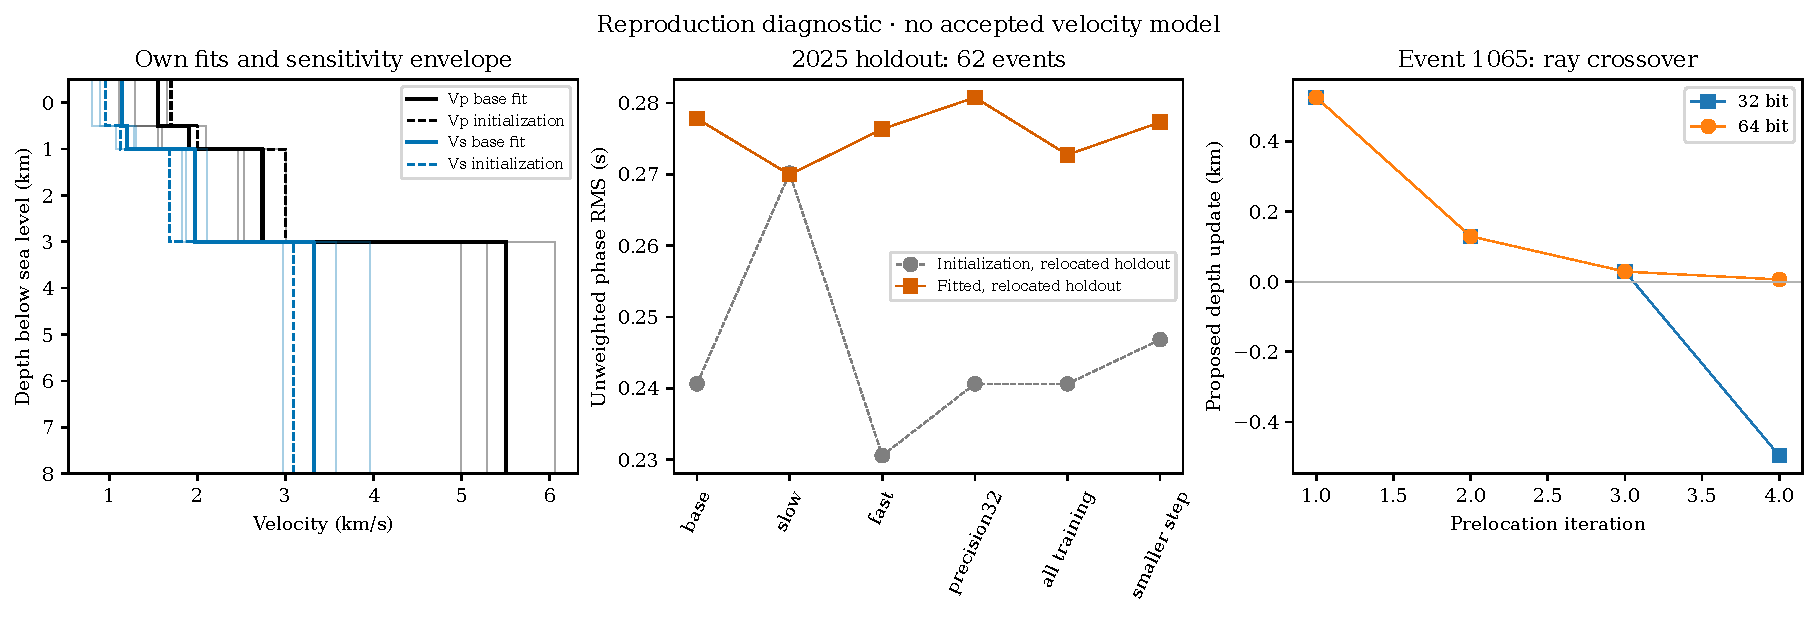
\includegraphics[width=\linewidth]{figures/observational_velocity_diagnostic.pdf}\end{center}

Reproduction diagnostic, not a publication panel. Dashed velocities are initialization; solid curves are independent provisional fits. The spread summarizes six specified sensitivity experiments. All residuals and depth steps are saved numerical results.

\par{\footnotesize\path{data/availability_extension/velocity_december/summary.json}}

\par{\footnotesize\path{data/availability_extension/velocity_december/sensitivity_profiles.csv}}

\par{\footnotesize\path{data/availability_extension/velocity_december/holdout_station_phase.csv}}

\par{\footnotesize\path{data/availability_extension/velocity_december/summary.json}}

\subsection*{Downstream scope and panel status}

The expanded cohort was also located in five fixed-model passes using the independently fitted base trial, with the documented 0.4/0.3 s residual rejection and final numerical filters. 1,414 of 3,018 initial causal events pass those filters. Figure S6 displays this unaccepted sensitivity calculation. Its model fails the holdout test; it is not promoted to a validated catalog. The earlier two-round fixed-grid relocations, magnitudes and mechanisms retain their earlier model and cohort and remain provisional.

\par{\footnotesize\path{data/availability_extension/catalog_december/locations_canonical/summary.json}}

Figures 2--4 and S7--S15 continue to identify their preserved numerical checkpoint unless an explicitly updated panel is listed. More raw files or isolated picks do not establish additional events, improved depths, completeness or reliable mechanisms. No published result table, catalog, pick, fitted velocity or digitized value fills a gap. Published figure images remain confined to the comparison PDF.

\subsection*{Rebuild and resume}

Use \path{scripts/rebuild_availability_extension.py} to verify the saved numerical checkpoint, regenerate its plots and compile both existing PDFs. Scientific commands and input placement are listed in \path{docs/AVAILABILITY_EXTENSION.md}. Acquisition and incremental picking have separate receipts; they are not counted as completed catalog analysis.

Earlier data/eida\_continuation and its plots remain preserved. The main manuscript, supplement, comparison layout, status record and document products are updated from saved results. Failed models and the original precision runs are retained. Reproduction remains partial; no panel is promoted to fully reproduced by this update.
